\documentclass[unicode]{beamer}
\usepackage{cmap}
\usepackage[T2A]{fontenc}
\usepackage[utf8]{inputenc}
\usepackage[english, russian]{babel}
\usepackage{amsmath,mathrsfs,amsfonts,amssymb}
\usepackage{graphicx, epsfig}
\usepackage{subfig}
\usepackage[noend]{algorithmic}

\usepackage{graphicx, epsfig}
\graphicspath{{pictures/}}
\DeclareGraphicsExtensions{.pdf,.png,.jpg}
\usepackage{subfig}
\usepackage{color}
\usepackage{gensymb}



\usepackage{algpseudocode}
\renewcommand{\algorithmicend}{\textbf{завершим}}
\renewcommand{\algorithmicif}{\textbf{если}}
\renewcommand{\algorithmicelse}{\textbf{иначе}}
\renewcommand{\algorithmicthen}{\textbf{то}}



\usetheme{Warsaw}%{Singapore}%{Warsaw}%{Warsaw}%{Darmstadt}
\usecolortheme{sidebartab}
\setbeamertemplate{footline}[author, institute]
\expandafter\def\expandafter\insertshorttitle\expandafter{%
  \insertshorttitle\hfill%
  \insertframenumber\,/\,\inserttotalframenumber}

% отключить клавиши навигации
\setbeamertemplate{navigation symbols}{}


\title[Модель альбедо снега]{Разработка математической модели расчета альбедо снега}
\author{Черненков Алексей}
\date{26 мая 2021 г.}
\institute[МФТИ(НИУ)]{Московский физико-технический институт \\ (национальный исследовательский университет) \\
    Физтех-школа Прикладной Математики и Информатики\\
    Кафедра вычислительных технологий и моделирования \\ в геофизике и биоматематике
    \vspace{0.3cm} \\
    Научный руководитель А.\,С.\,Грицун (С.\,В.\,Кострыкин)
}

\date{
    \footnotesize
    1 июля 2021 г.
}

\begin{document}

% Creates title page of slide show using above information
\begin{frame}
  \titlepage
\end{frame}



\begin{frame}{Постановка задачи}
    \footnotesize
    
    \begin{itemize}
    \item<1-2>[]\begin{block}{Альбедо}
        Альбедо -- это физическая величина, равная отношению отраженной от поверхности радиации к падающей 
        
        
    \end{block}
    
    \item<2->[]\begin{block}{Основные факторы, влияющие на альбедо}
        \begin{itemize}
            \item структура снега: форма и размеры снежных кристаллов
            \item наличие в снегу примесей 
            \item  солнечное склонение
        \end{itemize}
    \end{block}
    
    \end{itemize}

\end{frame}



\begin{frame}{Постановка задачи}
    \begin{itemize}
    \item<1-2>[]\begin{block}{Задача}
        Построить модель альбедо заснеженной поверхности, учитывающую зависимости от основных параметров, и пригодную для внедрения в глобальную климатическую модель, например, модель ИВМ РАН
    \end{block}
        
    \item<2->[]\begin{block}{Актуальность}
        Альбедо:
        \begin{itemize}
            \item важная переменная в климатических моделях
            \item участвует в описании радиационного баланса Земли
            \item уменьшение приводит к дополнительному нагреву поверхности
         \end{itemize}
    \end{block}
    \end{itemize}
\end{frame}



\begin{frame}{Этапы решения задачи}
    \footnotesize    
    
    \begin{itemize}
        \item<1-3>[]\begin{block}{Получение зависимостей, описывающих:}
            \begin{itemize}
                \item изменение солнечного зенитного угла в течении года
                \item метаморфизм снега
                \item концентрации примесей, содержащихся в снегу
            \end{itemize}
        \end{block}

        \item<2-3>[]\begin{block}{Модификация Климатической модели ИВМ РАН}
            Добавление в модель прогностических переменных, описывающих жидкую воду в слое снега, и лед, образовавшийся в результате перезамерзания талой воды, реализация расчета плотности слоя снега
        \end{block}
    
        \item<3->[]\begin{block}{Получение параметризации альбедо}
            Построение параметризации альбедо снега, зависящей от солнечного зенитного угла, размера снежного кристалла и концентрации примеси, на основании радиационной модели SNICAR
        \end{block}
    \end{itemize}

\end{frame}



\begin{frame}{Решение: солнечный зенитный угол}

\scriptsize
\begin{figure}[h]
    \begin{minipage}[h]{0.49\linewidth}
        \center{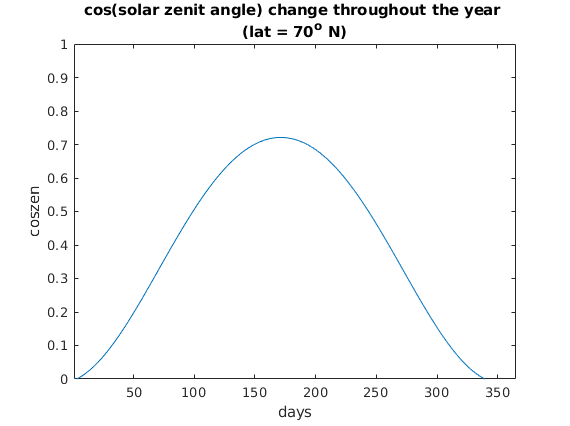
\includegraphics[width=1.1\linewidth]{coszen2.png} \\ (а)}
    \end{minipage}
    \begin{minipage}[h]{0.49\linewidth}
        \center{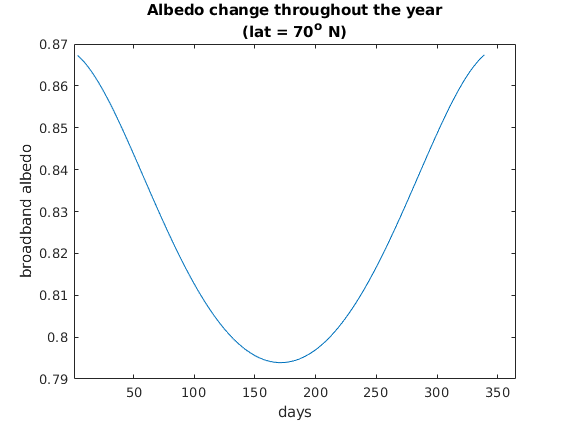
\includegraphics[width=1.1\linewidth]{coszen3.png} \\ (б)}
    \end{minipage}
\end{figure}
\center{Изменение (а) косинуса солнечного зенитного угла и (б) альбедо снега \\ в течении года, вызванные вращением Земли вокруг Солнца \\ (на примере точки на $70\degree$ С.Ш.)}

\end{frame}



\begin{frame}{Решение: солнечный зенитный угол}
    
Пусть $\delta$ –- угол склонения Солнца, $\phi$ –- широта, $\theta$ –- солнечный зенитный угол, тогда:
    \[\cos \theta = \cos ( \phi - \delta ), \]
при этом:
    \[\sin \delta = \sin \varepsilon \sin \left(\dfrac{2 \pi (d - d_e)}{365} \right), \]
где $\varepsilon$ = 23.45$\degree$  – наклон Земли к плоскости эклиптики, \\ $d$ – время (в сутках с начала года), $d_e$ = 80.5

\end{frame}



\begin{frame}{Решение: метаморфизм снега}

\scriptsize
\begin{figure}[h]
    \begin{minipage}[h]{0.44\linewidth}
        \center{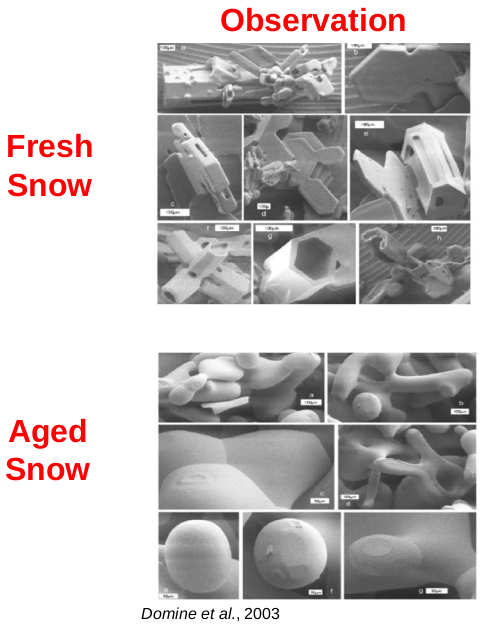
\includegraphics[width=1\linewidth]{aged_snow.png} }
    \end{minipage}
    \begin{minipage}[h]{0.55\linewidth}
        \center{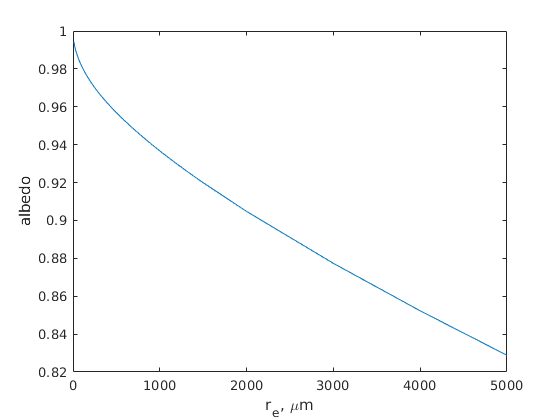
\includegraphics[width=1\linewidth]{rds2.png} \\ Зависимость альбедо \\ от эффективного радиуса \\ снежного кристалла}
    \end{minipage}
\end{figure}

\end{frame}



\begin{frame}{Решение: метаморфизм снега}

\scriptsize

\begin{itemize}
        \item Приближение ледяных шарообразных частиц, сохраняющих удельную площадь поверхности ($SSA$) 

        \item Основная характеристика приближения -- эффективный радиус $r_e$:
            \[ r_e = \dfrac{3} {\rho_{ice} \cdot SSA} \label{sys} \]
        \item Эволюция среднего по слою эффективного радиуса снежного кристалла\footnote{\scriptsize Community Land Model (CLM), version 4.5}:
        \footnotesize
        \begin{block}{}  
            \[ r_e(t) = [r_e (t - 1) + \delta r_{e , dry} + \delta r_{e , wet} ] \cdot f_{old} + r_{e ,0} \cdot f_{new} + r_{e , rfz} \cdot f_{rfrz} \]
        \end{block}    
        \scriptsize
        Здесь $ r_{e ,0} = 54.5 $ мкм и $r_{e , rfz} = 1000 $ мкм -- значения $r_e$, соответствующие свежевыпавшему и перезамерзшему снегу, $\delta r_{e , dry}$ и $\delta r_{e , wet}$ -- вклады от метаморфизма сухого и мокрого снега, $f_{old}$, $f_{new}$ и $f_{rfrz}$ -- доли лежалого, свежевыпавшего и перезамерзшего снега
\end{itemize}



\end{frame}



\begin{frame}{Решение: метаморфизм снега}

\footnotesize

\begin{itemize}
    \item Эволюция сухого снега описывается уравнением\footnote{\scriptsize Flanner and Zender, 2006}:
    \footnotesize
    \[ \dfrac{d}{dt} \delta r_{e , dry} = \gamma \cdot \left(\dfrac{\eta}{\eta + (r_e - r_{e, 0})}\right)^{1 / \kappa} \]
    $\gamma$, $\eta$, $\kappa$ -- табличные параметры, зависящие от $T$, $\dfrac{dT}{dz}$, $\rho_{snow}$

    \item Эволюция мокрого снега описывается эмпирическим законом\footnote{\scriptsize Brun, 1989}:
    \footnotesize
    \[ \dfrac{d}{dt} \delta r_{e , wet} = \dfrac{C \cdot f_{liq}^3} {4 \pi r_{e}^2} \]
    Здесь $C = 4.22 \cdot 10^{5}$ мкм$^3/$c, $f_{liq}$ -- доля жидкой воды в снегу
\end{itemize}

\end{frame}



\begin{frame}{Решение: метаморфизм снега}

\footnotesize

Объединяя уравнения для эволюции сухого и мокрого снега, получаем задачу Коши для суммарного вклада в метаморфизм из-за старения снега:
    \[ \begin{cases}
        \dfrac{d}{dt} \delta (r_{e , dry} + r_{e , wet}) = \gamma \cdot \left(\dfrac{\eta}{\eta + (r_e - r_{e, 0})}\right)^{1 / \kappa} + \dfrac{C \cdot f_{liq}^3} {4 \pi r_{e}^2} ,
        \\
        \delta (r_{e , dry} + r_{e , wet})(t_0) = 0; 
    \end{cases} \]

Данная задача решалась численно с помощью явного метода Эйлера

\end{frame}



\begin{frame}{Решение: загрязнение снега атмосферными аэрозолями}

\footnotesize
\begin{block}{}  
    Выпадая на заснеженную поверхность, атмосферные аэрозоли уменьшают ее отражающую способность, что приводит к дополнительному нагреву и ускоренному таянию
\end{block} 


\scriptsize
\begin{figure}[h]
    \begin{minipage}[h]{0.49\linewidth}
        \center{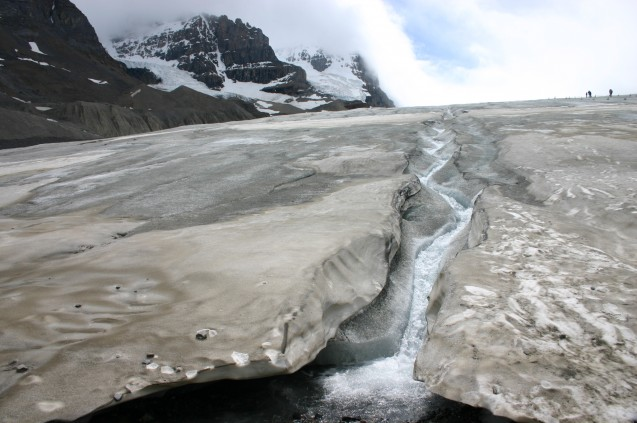
\includegraphics[width=1\linewidth]{Melting_Glacier.jpg} Тающий ледник Атабаска в Канаде \\ (ph. Wing-Chi Poon)}
    \end{minipage}
    \begin{minipage}[h]{0.5\linewidth}
        \center{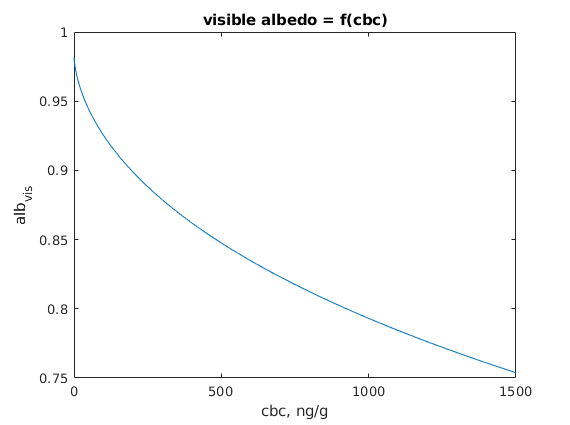
\includegraphics[width=1\linewidth]{alb_cbc.png} \\ Зависимость альбедо от \\ концентрации ЧУ в снегу}
    \end{minipage}
\end{figure}


\end{frame}



\begin{frame}{Решение: загрязнение снега атмосферными аэрозолями}

\footnotesize
\begin{itemize}
    \item Масса ЧУ в заснеженной ячейке сетки описывается балансовым соотношением:
    \[ \dfrac{d M_{bc}}{d t} = - C_{MSE} Q_{melt} \dfrac{M_{bc}}{M_{sn}} ~ S + I_{bc} \sigma S \]
    \item Уравнение баланса в дискретном виде:
    \[ M_{bc}^{n+1} = M_{bc}^n - C_{MSE} ~ Q_{melt}^{n+1} ~ \dfrac{M_{bc}^n}{M_{sn}^n} ~ S \Delta t + P_{bc}^{n+1} \]
    \item Начальные условия задаются в момент появления снежного покрова в данной ячейке сетки:
    \[ M_{bc}^0 = P_{bc}^0 \]
    \item Зная решение балансового уравнения, можно найти концентрацию ЧУ в снегу:
    \[ C_{bc}^n = \dfrac{M_{bc}^n}{M_{sn}^n} \]
\end{itemize}

\end{frame}



\begin{frame}{Решение: загрязнение снега атмосферными аэрозолями}

\tiny
\begin{figure}[h]
    \begin{minipage}[h]{0.85\linewidth}
        \center{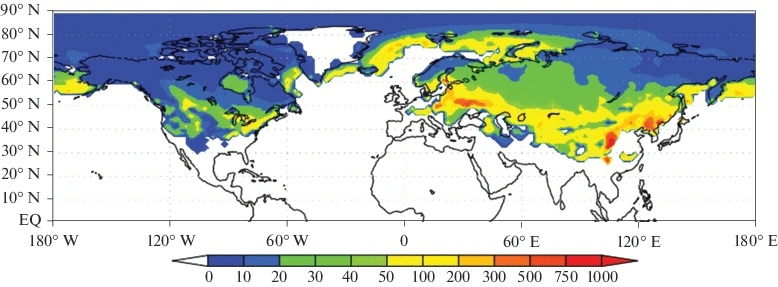
\includegraphics[width=1\linewidth]{Cbc1.jpg} \\ Среднемесячная концентрация черного углерода в снегу, рассчитанная по данным климатической модели ИВМ РАН (январь 1998 г.), [нг/г]\\
    \footnotesize
    ~\\
    \\}
    \end{minipage}
    
    \begin{minipage}[h]{1\linewidth}
        \\
        ~\\
        \\
        \center{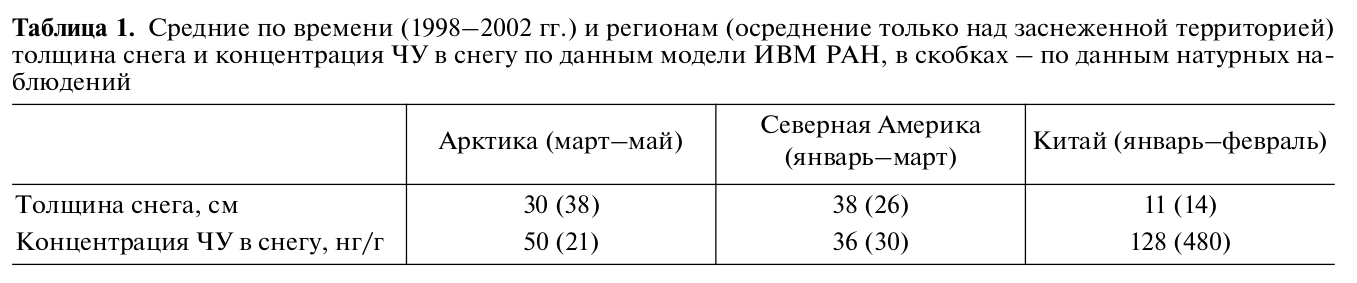
\includegraphics[width=1\linewidth]{table1.png} }
    \end{minipage}
\end{figure}

\end{frame}



\begin{frame}{Решение: модификация климатической модели ИВМ РАН}

\footnotesize
Для совместного использования модели альбедо, учитывающей старение снега, и глобальной климатической модели ИВМ РАН были необходимы следующие изменения в почвенно-снежном блоке модели:

\begin{itemize}
    \item  модификация процесса таяния снега 
    \item  реализация процесса перезамерзания талой воды
    \item  реализация эволюции плотности снега с учетом новых процессов
\end{itemize}

\end{frame}



\begin{frame}{Решение: модификация климатической модели ИВМ РАН}

\scriptsize
\begin{figure}[h]
    \begin{minipage}[h]{0.48\linewidth}
        \center{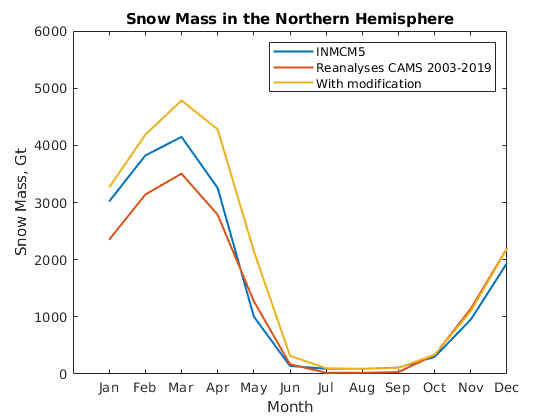
\includegraphics[width=1.1\linewidth]{snow_mass.png} \\ (а) }
    \end{minipage}
    \hfill
    \begin{minipage}[h]{0.51\linewidth}
        \center{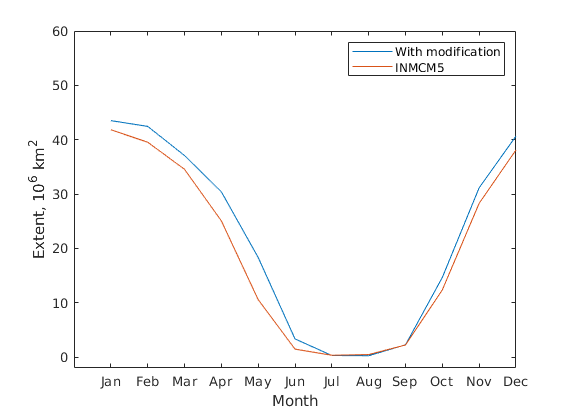
\includegraphics[width=1.1\linewidth]{snow_square.png} \\ (б) }
    \end{minipage}
\end{figure}
\center{Годовой ход (а) массы снега и (б) площади, покрытой им, осредненные за 1997-2002 годы по данным исходной и модифицированной версий модели, и по данным реанализа CAMS за 2003--2019 годы}

\end{frame}



\begin{frame}{Решение: параметризация альбедо на основе модели SNICAR}

\footnotesize

Ищется параметризация альбедо снега следующего вида: 
    \[ albedo = f(r_e, C_{bc}, coszen) \]
\\
На первом этапе предлагается искать параметризацию альбедо в виде полинома от двух переменных, полагая $coszen = 1$:
    \[ alb_1(r_e, C_{bc}) = \sum_{i,j = 0}^N \sigma_{i.j} r_e^i C_{bc}^j  \]
    \
    \scriptsize Установлено, что наилучший результат достигается в случае $N = 5$
    \footnotesize
\\
~\\
\\
На втором этапе альбедо уточняется на основании эмпирической  зависимости\footnote{\scriptsize Saito, 2019}:
    \footnotesize
    \[ alb(r_e, C_{bc}, coszen) = \alpha + (A + B \cdot \alpha^C) \left( \dfrac{1 - coszen}{1 + coszen} \right)^D \]
    \center{\tiny ($\alpha = alb_1(r_e, C_{bc})$ -- приближение с первого шага)}


\\
\scriptsize
\begin{flushright}
    Параметры $\{ \sigma_{i.j} \}, A, B, C, D$ находятся из результатов запусков модели SNICAR на различных наборах входных данных
\end{flushright}

\end{frame}



\begin{frame}{Расчеты с использованием разработанной модели альбедо}

%\scriptsize
\tiny
\begin{figure}[h]
    \begin{minipage}[h]{0.63\linewidth}
        \center{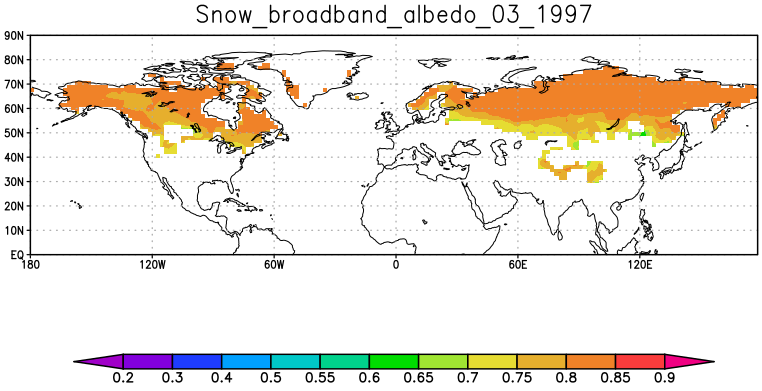
\includegraphics[width=1\linewidth]{Snow_albedo_03_1997.png} Среднемесячное широкополосное альбедо заснеженной поверхности, рассчитанное с помощью построенной модели альбедо (март 1997 г.) \\~}
    \end{minipage}
    \\~
    \begin{minipage}[h]{0.63\linewidth}
        \center{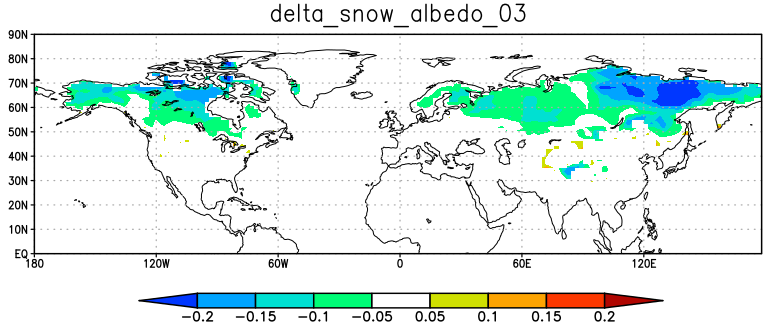
\includegraphics[width=1\linewidth]{delta_snow_albedo_03.png} Разность альбедо по данным реанализа CAMS и рассчитанного с помощью построенной модели (месяц март)}
    \end{minipage}
\end{figure}

\end{frame}



\begin{frame}{Заключение}

%\footnotesize
\begin{itemize}
    \item Разработана модель альбедо снега
    
    \item Модифицирован почвенно-снежный блок глобальной климатической модели ИВМ РАН, улучшено воспроизведение площади, покрытой снегом, в сравнении с данными реанализа 
    
    \item Полученную модель можно использовать для внедрения блока расчета альбедо в модель климата
    
    \item Полученную модель можно использовать для оффлайн-оценки радиационного форсинга от загрязнения снега атмосферными аэрозолями 
\end{itemize}    
    
\end{frame}



\begin{frame}{Заключение}


\footnotesize
Отдельные результаты магистерской диссертации изложены в статье:
\tiny
\begin{itemize}    
    \item А.Ю. Черненков, С.В. Кострыкин, Оценка радиационного форсинга от загрязнения снега черным углеродом по данным климатической модели, Известия РАН. Физика атмосферы и океана, 2021, T.57, №2, стр. 146-155, DOI: 10.31857/S0002351521020036. 
\end{itemize} 

\footnotesize
а также докладывались и обсуждались на следующих научных конференциях, в том числе с международным участием:
\tiny
\begin{itemize}
    \item Международный симпозиум «Атмосферная радиация и динамика» (МСАРД–2019), 25 – 27 июня 2019, Санкт-Петербург.
    \item 62-я Всероссийская научная конференция МФТИ, секция ФПМИ – Вычислительные технологии и моделирование, Москва, 2019.
    \item EGU2020: Sharing Geoscience Online, ITS2.15/BG2.25 Pan-Eurasian Experiment (PEEX) – Observation, Modelling and Assessment in the Arctic-Boreal Domain, May, 2020.\sloppy 
    \item 63-я Всероссийская научная конференция МФТИ, Секция ФПМИ – Вычислительные технологии и моделирование, Москва, 2020.
    \item Вторая Всероссийская научная конференция «Мониторинг состояния и загрязнения окружающей среды. Экосистемы и климат Арктической зоны». Москва, 25-27 ноября 2020г.
\end{itemize} 
\end{frame}



\begin{frame}{}
\begin{center}
    \Large{Спасибо за внимание!}
\end{center}
\end{frame}



\begin{frame}{Дополнение 1: модификация климатической модели ИВМ РАН}

\footnotesize

\begin{itemize}
    \item $S$ -- водно-эквивалентная толщина слоя снега
    \item $S_{sn}$ -- "настоящий"\  снег (по сути, крошка из пористого льда) 
    \item $M_{soil}$ -- вода, поступившая на поверхность почвы
    \item $P$ -- интенсивность осадков при температуре подстилающей поверхности, меньшей $0 ~\degree$C
    \item $\lambda$ -- удельная теплота плавления льда 
    \item $\mathcal{L}$ -- удельная теплота парообразования 
    \item $\mathcal{E}$ -- поток скрытого тепла на поверхность снега, идущего на испарение/сублимацию
    \item $\rho_w$ -- плотность воды
    \item $M$ -- интенсивность снеготаяния
    \item $S_{wat}$ -- талая вода, оставшаяся в слое снега
    \item $F$ -- интенсивность замерзания воды
    \item $S_{rfrz}$ -- перезамерзшая талая вода (по сути, крошка из плотного льда)
    \item $T_{sn}$ -- температура снега
    \item $\Delta E$ -- избыточный/дефицитный поток тепла в тепловом балансе на поверхности
\end{itemize}

\end{frame}



\begin{frame}{Дополнение 1: модификация климатической модели ИВМ РАН}

\tiny

    \If{$ \Delta E >0$, $T_{sn} = 0 ~\degree$C и $S^{n-1} > 0 $}
        \State $ M = \dfrac{\Delta E}{\lambda} $, ~ $ \delta = \dfrac{S_{sn}^{n-1}}{S_{sn}^{n-1} + S_{rfrz}^{n - 1}}$ 
        \State $ S_{sn}^n = S_{sn}^{n-1} + P - \Delta t \left( \dfrac{\mathcal{E}}{\mathcal{L} \cdot \rho_w} + \delta \cdot M \right) $, ~  $ S_{wat}^{max} = f( S_{sn}^n ) $
        \State $ S_{rfrz}^n = S_{rfrz}^{n - 1} - \Delta t (1 - \delta)M $ 
        \State $ \Delta S_{wat} = max\{\Delta t \cdot M, ~S_{wat}^{max}\} $, ~ $ M_{soil} = max\{\Delta t \cdot M - S_{wat}^{max}, ~0\} $ 
        \State $ S_{wat}^n = S_{wat}^{n-1} + \Delta S_{wat} $ 
    \Else
        \If{$S^{n-1} > 0$, $S_{wat}^{n-1} > 0$ и $T_{sn} = 0 ~\degree$C}
            \State $F = -\dfrac{\Delta E}{\lambda}$, ~ $S_{sn}^n = S_{sn}^{n-1} + P - \Delta t \left( \dfrac{\mathcal{E}}{\mathcal{L} \cdot \rho_w} - F \right)$
            \State $S_{rfrz}^n = S_{rfrz}^{n - 1} + ( S_{wat}^{n-1} - S_{wat}^n )$
            \State $S_{wat}^n = max\{ S_{wat}^{n-1} - \Delta t \cdot F, ~0\}$
        \EndIf
    \EndIf
    \State $S^n = S_{sn}^n + S_{wat}^n + S_{rfrz}^n$

\end{frame}



\begin{frame}{Дополнение 1: модификация климатической модели ИВМ РАН}

\footnotesize
Основные изменения:

\begin{itemize}
    \item  В случае фазовых переходов избыток энергии в тепловом балансе на поверхности тратится на таяние снега, а дефицит восполняется 
    \item  Талая вода не уходит моментально на верхнюю границу почвы, сочится сквозь толщу снега. При этом в слое снега может содержаться воды не больше критического значения $S_{wat}^{max}$
    \item Критическая масса воды $S_{wat}^{max}$, способная содержаться в слое снега, зависит от водно-эквивалентной высоты снежного покрова $S$ и его пористости $\varepsilon_{sn}$:
    \[ S_{wat}^{max} = S ~\dfrac{\varepsilon_{sn}}{1 - \varepsilon_{sn}} \]
    \item Пористость снега определяется с его плотностью:
    \[ \varepsilon_{sn} = 0.11 \left( \dfrac{\rho_w}{\rho_{sn}} - 1 \right) \]

\end{itemize}

\end{frame}



\begin{frame}{Дополнение 1: модификация климатической модели ИВМ РАН}

\footnotesize

\begin{itemize}
    \item  Эволюция плотности лежалого снега задается уравнением:
    \begin{block}{}    
    \[ \rho_{sn}(\tau_i) = \rho_{sn}(\tau_{i-1}) \left[  1 + 0.1 H_{sn}(\tau_{i-1}) \exp \{ 0.08 T_{sn} - 21 \rho_{sn}(\tau_{i-1})  \} \right] \]
    \end{block}
    \scriptsize
    Здесь $H_{sn}$ -- водно-эквивалентная толщина слоя снега в см, плотность снега $\rho_{sn}$ в г/см$^3$, температура слоя снега $T_{sn}$ в $\degree$C, шаг по времени $\tau_{i} - \tau_{i-1} = 1$ сутки, поэтому для использования в модели ИВМ необходима переинтерполяция
    \footnotesize
    \item  Слой снега может состоять из лежалого, свежевыпавшего или перезамерзшего снега, содержать талую воду, поэтому плотность снежного слоя рассчитывается как среднее взвешенное по всем этим фракциям:
    \begin{block}{}    
    \[ \rho_{snow} = \rho_{old} \cdot \delta_{old} + \rho_{new} \cdot \delta_{new} + \rho_{w} \cdot \delta_{wat} + \rho_{ice} \cdot \delta_{rfrz} \]
    \end{block}
    \scriptsize
    Здесь $\rho_{old}$ -- плотность лежалого снега,  $\rho_{new} = 0.1$ г/см$^3$ -- плотность свежевыпавшего снега, $\rho_{w} = 1$ г/см$^3$ -- плотность воды, $\rho_{ice} = 0.917$ г/см$^3$ -- плотность льда, $\delta_{old}, ~\delta_{new}, ~\delta_{wat}, ~\delta_{rfrz}$ -- массовые доли старого и свежего снега, талой воды, а также перезамерзшего снега
\end{itemize}

\end{frame}


\begin{frame}{Дополнение 2: применение модели альбедо для вычисления радиационного форсинга}

\footnotesize
Пусть:
\begin{itemize}
    \item $\alpha_{0}$ и $\alpha_{soot}$ -- альбедо чистого и загрязненного снега соответственно,
    \item $\alpha^{vis}$ -- величина альбедо, соответствующая излучению в видимом диапазоне ($0.3-0.7$ мкм),
    \item $\alpha^{nir}$ -- величина альбедо, соответствующая излучению в ближнем ИК диапазоне ($0.7-5.0$ мкм),
    \item $\sigma$ -- доля области, покрытая снегом,
    \item $F_{sw}$ -- поток приходящей коротковолновой радиации
\end{itemize}
Тогда форсинг можно оценить по следующей формуле:
    \[ R = \sigma [ (\alpha_{0}^{vis} - \alpha_{soot}^{vis})F_{down}^{vis} + (\alpha_{0}^{nir} - \alpha_{soot}^{nir})F_{down}^{nir} ] \]
При этом, потоки радиации $F_{down}^{vis}$ и $F_{down}^{nir}$ можно оценить следующим образом: 
\[ F_{down}^{vis} \approx F_{down}^{nir} \approx 0.5 \cdot F_{sw} \]
    
\end{frame}



\begin{frame}{Дополнение 2: применение модели альбедо для вычисления радиационного форсинга}

\scriptsize
\begin{figure}[h]
    \center{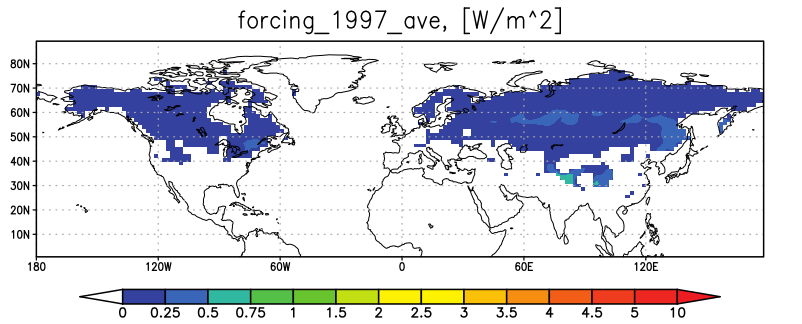
\includegraphics[scale=0.3]{forcing_1997.png}}
\end{figure}
\center{Среднегодовой радиационный форсинг из-за загрязнения снега черным углеродом, рассчитанный с помощь построенной модели альбедо (1997 г.)}    

\end{frame}



\end{document}